\chapter{Joshua 11}

\begin{figure}
  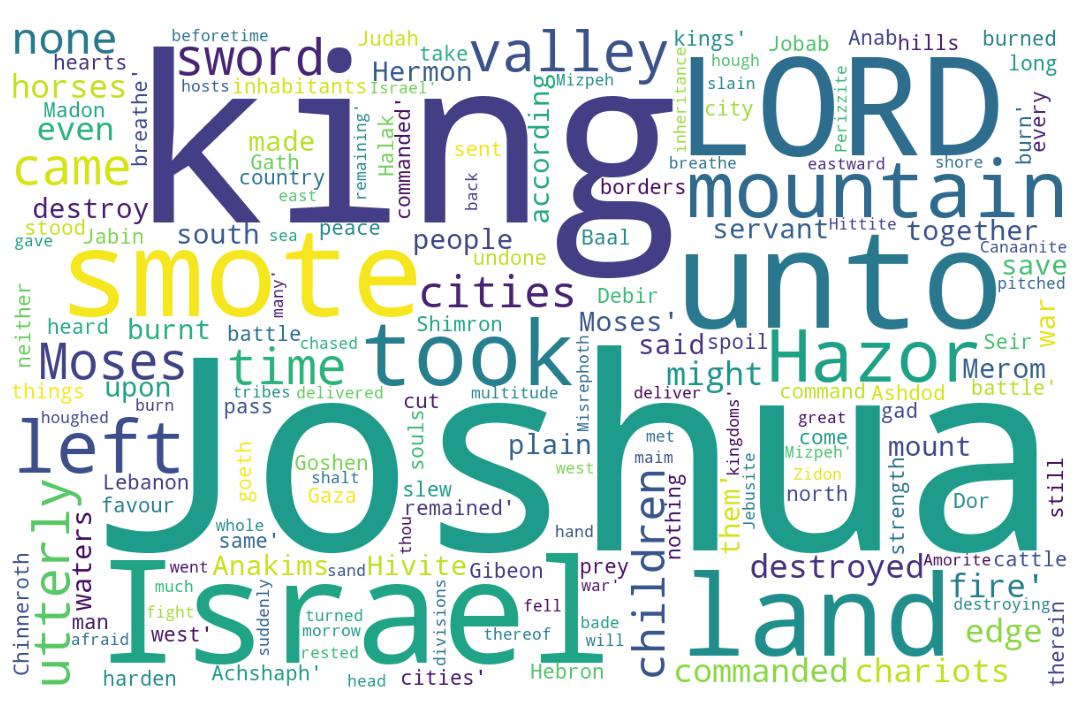
\includegraphics[width=\linewidth]{06OT-Joshua/Joshua11-WordCloud.jpg}
  \caption{Joshua 11 Word Cloud}
  \label{fig:Joshua 11 Word Cloud}
\end{figure}

\marginpar{\scriptsize \centering \fcolorbox{bone}{lime}{\textbf{THE SOUTHERN CAMPAIGN}}\\ (Joshua 11) \begin{compactenum}[I.][8]
	\item \textbf{Responisbility to Fight} \index[scripture]{Joshua!Jsh 11:01}  (Jsh 11:1) 
	\item The Enemy's \textbf{Resources} \index[scripture]{Joshua!Jsh 11:04}  (Jsh 11:4)
	\item The Enemy's \textbf{Resistance} \index[scripture]{Joshua!Jsh 11:05}  (Jsh 11:5)
	\item The \textbf{Readiness} to Fight the Long Battles \index[scripture]{Joshua!Jsh 11:18}  (Jsh 11:18)
	\item The \textbf{Reknowned} Giants \index[scripture]{Joshua!Jsh 11:21}  (Jsh 11:21)
	\item  Where the Enemy \textbf{Remained}  \index[scripture]{Joshua!Jsh 11:22}  (Jsh 11:22)
	\item  \textbf{Rest} in the Land \index[scripture]{Joshua!Jsh 11:23}  (Jsh 11:23)
\end{compactenum}}




\footnote{\textcolor[rgb]{0.00,0.25,0.00}{\hyperlink{TOC}{Return to end of Table of Contents.}}}\footnote{\href{https://audiobible.com/bible/joshua_11.html}{\textcolor[cmyk]{0.99998,1,0,0}{Joshua 11 Audio}}}\textcolor[cmyk]{0.99998,1,0,0}{\fcolorbox{bone}{bone}{And} it came \fcolorbox{bone}{bone}{to} pass, when Jabin king of Hazor had heard \emph{those} \emph{things}, that he sent \fcolorbox{bone}{bone}{to} Jobab king of Madon, and \fcolorbox{bone}{bone}{to} the king of Shimron, and \fcolorbox{bone}{bone}{to} the king of Achshaph,}
[2] \textcolor[cmyk]{0.99998,1,0,0}{\fcolorbox{bone}{bone}{And} \fcolorbox{bone}{bone}{to} the kings that \emph{were} on the north of the mountains, and of the plains south of Chinneroth, and \fcolorbox{bone}{bone}{in} the valley, and \fcolorbox{bone}{bone}{in} the borders of Dor on the west,}
[3] \textcolor[cmyk]{0.99998,1,0,0}{\emph{And} \emph{to} the Canaanite on the east and on the west, and \emph{to} the Amorite, and the Hittite, and the Perizzite, and the Jebusite \fcolorbox{bone}{bone}{in} the mountains, and \emph{to} the Hivite under Hermon \fcolorbox{bone}{bone}{in} the land of Mizpeh.}
[4] \textcolor[cmyk]{0.99998,1,0,0}{\fcolorbox{bone}{bone}{And} \fcolorbox{bone}{bone}{they} went out, \fcolorbox{bone}{bone}{they} and all their hosts \fcolorbox{bone}{bone}{with} them, much people, even as the sand that \emph{is} upon the sea shore \fcolorbox{bone}{bone}{in} multitude, \fcolorbox{bone}{bone}{with} horses and chariots very many.}
[5] \textcolor[cmyk]{0.99998,1,0,0}{\fcolorbox{bone}{bone}{And} when all these kings were met together, \fcolorbox{bone}{bone}{they} came and pitched together at the waters of Merom, \fcolorbox{bone}{bone}{to} fight against Israel.}\\
\\
\P \textcolor[cmyk]{0.99998,1,0,0}{\fcolorbox{bone}{bone}{And} the LORD said unto Joshua, Be not afraid because of them: for \fcolorbox{bone}{bone}{to} morrow about this time will I deliver them up all slain before Israel: thou shalt hough their horses, and burn their chariots \fcolorbox{bone}{bone}{with} fire.}
[7] \textcolor[cmyk]{0.99998,1,0,0}{So Joshua came, and all the people of war \fcolorbox{bone}{bone}{with} him, against them by the waters of Merom suddenly; and \fcolorbox{bone}{bone}{they} fell upon them.}
[8] \textcolor[cmyk]{0.99998,1,0,0}{\fcolorbox{bone}{bone}{And} the LORD delivered them into the hand of Israel, who smote them, and chased them unto great Zidon, and unto Misrephoth-maim, and unto the valley of Mizpeh eastward; and \fcolorbox{bone}{bone}{they} smote them, until \fcolorbox{bone}{bone}{they} left them none remaining.}
[9] \textcolor[cmyk]{0.99998,1,0,0}{\fcolorbox{bone}{bone}{And} Joshua did unto them as the LORD bade him: he houghed their horses, and burnt their chariots \fcolorbox{bone}{bone}{with} fire.}\\
\\
\P \textcolor[cmyk]{0.99998,1,0,0}{\fcolorbox{bone}{bone}{And} Joshua at that time turned back, and took Hazor, and smote the king thereof \fcolorbox{bone}{bone}{with} the sword: for Hazor beforetime was the head of all those kingdoms.}
[11] \textcolor[cmyk]{0.99998,1,0,0}{\fcolorbox{bone}{bone}{And} \fcolorbox{bone}{bone}{they} smote all the souls that \emph{were} therein \fcolorbox{bone}{bone}{with} the edge of the sword, utterly destroying \emph{them}: there was not any left \fcolorbox{bone}{bone}{to} breathe: and he burnt Hazor \fcolorbox{bone}{bone}{with} fire.}
[12] \textcolor[cmyk]{0.99998,1,0,0}{\fcolorbox{bone}{bone}{And} all the cities of those kings, and all the kings of them, did Joshua take, and smote them \fcolorbox{bone}{bone}{with} the edge of the sword, \emph{and} he utterly destroyed them, as Moses the servant of the LORD commanded.}
[13] \textcolor[cmyk]{0.99998,1,0,0}{But \emph{as} \emph{for} the cities that stood still \fcolorbox{bone}{bone}{in} their strength, Israel burned none of them, save Hazor only; \emph{that} did Joshua burn.}
[14] \textcolor[cmyk]{0.99998,1,0,0}{\fcolorbox{bone}{bone}{And} all the spoil of these cities, and the cattle, the children of Israel took for a prey unto themselves; but every man \fcolorbox{bone}{bone}{they} smote \fcolorbox{bone}{bone}{with} the edge of the sword, until \fcolorbox{bone}{bone}{they} had destroyed them, neither left \fcolorbox{bone}{bone}{they} any \fcolorbox{bone}{bone}{to} breathe.}\\
\\
\P \textcolor[cmyk]{0.99998,1,0,0}{As the LORD commanded Moses his servant, so did Moses command Joshua, and so did Joshua; he left nothing undone of all that the LORD commanded Moses.}
[16] \textcolor[cmyk]{0.99998,1,0,0}{So Joshua took all that land, the hills, and all the south country, and all the land of Goshen, and the valley, and the plain, and the mountain of Israel, and the valley of the same;}
[17] \textcolor[cmyk]{0.99998,1,0,0}{\emph{Even} from the mount Halak, that goeth up \fcolorbox{bone}{bone}{to} Seir, even unto Baal-gad \fcolorbox{bone}{bone}{in} the valley of Lebanon under mount Hermon: and all their kings he took, and smote them, and slew them.}
[18] \textcolor[cmyk]{0.99998,1,0,0}{Joshua made war a long time \fcolorbox{bone}{bone}{with} all those kings.}
[19] \textcolor[cmyk]{0.99998,1,0,0}{There was not a city that made peace \fcolorbox{bone}{bone}{with} the children of Israel, save the Hivites the inhabitants of Gibeon: all \emph{other} \fcolorbox{bone}{bone}{they} took \fcolorbox{bone}{bone}{in} battle.}
[20] \textcolor[cmyk]{0.99998,1,0,0}{For it was of the LORD \fcolorbox{bone}{bone}{to} harden their hearts, that \fcolorbox{bone}{bone}{they} should come against Israel \fcolorbox{bone}{bone}{in} battle, that he might destroy them utterly, \emph{and} that \fcolorbox{bone}{bone}{they} might have no favour, but that he might destroy them, as the LORD commanded Moses.}\\
\\
\P \textcolor[cmyk]{0.99998,1,0,0}{\fcolorbox{bone}{bone}{And} at that time came Joshua, and cut off the Anakims from the mountains, from Hebron, from Debir, from Anab, and from all the mountains of Judah, and from all the mountains of Israel: Joshua destroyed them utterly \fcolorbox{bone}{bone}{with} their cities.}
[22] \textcolor[cmyk]{0.99998,1,0,0}{There was none of the Anakims left \fcolorbox{bone}{bone}{in} the land of the children of Israel: only \fcolorbox{bone}{bone}{in} Gaza, \fcolorbox{bone}{bone}{in} Gath, and \fcolorbox{bone}{bone}{in} Ashdod, there remained.}
[23] \textcolor[cmyk]{0.99998,1,0,0}{So Joshua took the whole land, according \fcolorbox{bone}{bone}{to} all that the LORD said unto Moses; and Joshua gave it for an inheritance unto Israel according \fcolorbox{bone}{bone}{to} their divisions by their tribes. \fcolorbox{bone}{bone}{And} the land rested from war.}